\documentclass[UTF8]{ctexart}
\usepackage{amsmath}
\usepackage{booktabs}
\usepackage{geometry}
\usepackage{listings}
\usepackage{xcolor}
\usepackage{hyperref}
\usepackage{graphicx}
\usepackage{float}

\geometry{a4paper, left=2.5cm, right=2.5cm, top=2.5cm, bottom=2.5cm}
\hypersetup{colorlinks=true, linkcolor=blue, urlcolor=blue, citecolor=blue}

\lstset{
  basicstyle=\ttfamily\small,
  breaklines=true,
  frame=single,
  keywordstyle=\color{blue},
  commentstyle=\color{gray},
  stringstyle=\color{teal},
  showstringspaces=false,
  tabsize=2,
  columns=flexible,
}

\title{\textbf{系统工具开发课程实验报告（第一周）}}
\author{廖世嘉 \quad 25020007073 \\ 25级计算机科学与技术}
\date{2026年8月24日}

\begin{document}
\maketitle
\tableofcontents
\newpage

\section{实验基本信息}

\begin{table}[H]
\centering
\caption{实验基本信息}
\label{tab:info}
\begin{tabular}{ll}
\toprule
项目 & 内容 \\
\midrule
姓名 & 廖世嘉 \\
学号 & 25020007073 \\
专业 & 25级计算机科学与技术 \\
实验环境 & Linux / Bash / Git / XeLaTeX \\
课上实验 & 4 个（含空格文件名整理、日志统计、Git 合并冲突、LaTeX 文档构建）\\
课后练习 & 16 个（Shell 基础、管道文本处理、Git 版本控制等）\\
GitHub仓库 & \href{https://github.com/MrLLLiao/SystemToolkitDevCourse}{https://github.com/MrLLLiao/SystemToolkitDevCourse} \\
\bottomrule
\end{tabular}
\end{table}

\section{实验目的}

本实验围绕 Shell 基础与文件系统、Shell 管道与文本处理、Git 版本控制以及 LaTeX 文档编辑四个主题展开。
课上完成四个连续实验，熟悉命令行环境下的文件操作、脚本编写、日志分析、分支管理、冲突解决和技术文档构建方法；
通过命令行验证文件权限、脚本退出码、Git 工作区状态以及 PDF 交叉引用，形成完整的"操作——验证——排错"实践流程。
课后通过 16 个练习进一步夯实 Shell 引号、通配符、重定向、退出码、权限与调试等基础，
并深入 Git 数据模型、历史可视化、stash 与冲突解决等版本控制知识。

\section{实验环境与工具}

本实验在 Linux 环境中完成，主要使用 Bash、find、ls、cp、chmod、awk、sort、head、Git、XeLaTeX/latexmk、
pdftotext 与 file 等工具。课上实验位于 week1/q01--q04，课后练习位于 week1/homework/q01--q16。
实验中全程遵守"分步提交、禁止单次全量提交"的 Git 规范，每个练习一个独立 commit。

% ================= 第一部分：课上实验 =================

\section{课上实验一：含空格文件名的批量整理}

\subsection{实验要求}

在 q01 中创建 input/docs 和 input/tmp，并创建 notes one.txt（内容为 alpha 和 beta 两行）、
隐藏文件 .secret.txt（内容为 hidden）、空文件 empty.txt 以及两行日志。
随后将所有 .txt 文件复制到 work/25020007073，保持相对目录结构，并将目录权限设为 750、
普通文件权限设为 640，最后生成 inventory.txt 列出相对路径和字节数。

\subsection{主要操作}

使用 mkdir -p 创建目录，利用 printf 和 touch 创建文件。对于包含空格的文件名，
在 Shell 中使用引号包围整个路径：

\begin{lstlisting}[language=bash]
printf "alpha\nbeta\n" > "input/docs/notes one.txt"
printf "hidden\n" > input/docs/.secret.txt
touch input/tmp/empty.txt
printf "INFO: program started\nINFO: program finished\n" > input/run.log
\end{lstlisting}

使用 ls -laR input 以长格式递归显示全部项目，其中 -a 保证隐藏文件能够显示。
复制文件时使用 find ... -print0 配合 read -d ''，避免文件名中的空格导致错误分割：

\begin{lstlisting}[language=bash]
STUDENT_ID="25020007073"
mkdir -p "work/$STUDENT_ID"
find input -type f -name "*.txt" -print0 |
while IFS= read -r -d '' file; do
  relative="${file#input/}"
  mkdir -p "work/$STUDENT_ID/$(dirname "$relative")"
  cp -- "$file" "work/$STUDENT_ID/$relative"
done
\end{lstlisting}

然后使用 find 配合 chmod 设置权限：

\begin{lstlisting}[language=bash]
find "work/$STUDENT_ID" -type d -exec chmod 750 {} +
find "work/$STUDENT_ID" -type f -exec chmod 640 {} +
\end{lstlisting}

生成清单：

\begin{lstlisting}[language=bash]
find "work/$STUDENT_ID" -type f ! -name "inventory.txt" \
  -printf '%P\t%s\n' > "work/$STUDENT_ID/inventory.txt"
chmod 640 "work/$STUDENT_ID/inventory.txt"
\end{lstlisting}

\subsection{结果与验证}

实际检查结果表明，input 下正确存在 notes one.txt、.secret.txt、empty.txt 和 run.log。
其中前三个文本文件的大小分别为 11、7 和 0 字节。复制后的 work/25020007073 中，
目录显示为 drwxr-x---，即 750；普通文件显示为 -rw-r-----，即 640。
inventory.txt 成功记录复制后的相对路径和字节数：

\begin{lstlisting}
tmp/empty.txt 0
docs/.secret.txt 7
docs/notes one.txt 11
\end{lstlisting}

% ================= 课上实验二 =================

\section{课上实验二：随机访问日志统计}

\subsection{实验要求}

在 q02 中创建给定的 CSV 数据并编写 analyze.sh。脚本接收 CSV 路径，若文件不存在则将错误写入标准错误
并返回非零退出码；正常情况下使用 Shell 管道、awk、sort、head 统计 HTTP 5xx 次数最多的前两个 path，
并计算全部数据行的平均延迟。

\subsection{脚本实现}

文件检查部分如下：

\begin{lstlisting}[language=bash]
file="$1"
if [ -z "$file" ]; then
  echo "Error: missing CSV file path" >&2
  exit 1
fi
if [ ! -f "$file" ]; then
  echo "Error: file not found: $file" >&2
  exit 1
fi
\end{lstlisting}

5xx 统计通过 awk 对状态码进行过滤，再通过 sort 和 head 完成排序与截取：

\begin{lstlisting}[language=bash]
awk -F',' 'NR > 1 && $4 ~ /^5[0-9][0-9]$/ { count[$3]++ }
END { for (path in count) print count[path], path }' "$file" |
sort -k1,1nr -k2,2 |
head -n 2
\end{lstlisting}

sort -k1,1nr 负责按次数数值降序排列，-k2,2 在次数相同时按路径字典序排列。
平均延迟通过另一个 awk 忽略表头并保留两位小数：

\begin{lstlisting}[language=bash]
awk -F',' 'NR > 1 { sum += $5; count++ }
END { printf "%.2f\n", sum / count }' "$file"
\end{lstlisting}

\subsection{结果}

运行 ./analyze.sh access.csv 得到：

\begin{lstlisting}
Top 2 5xx paths:
2 /api/orders
2 /api/users
Average latency_ms:
193.75
\end{lstlisting}

运行不存在的文件时，脚本输出文件不存在错误并返回退出码 1，说明标准错误和非零退出状态处理符合要求。
本实验未使用 Python、电子表格或手工统计。

% ================= 课上实验三 =================

\section{课上实验三：制造、解决并解释一次 Git 合并冲突}

\subsection{实验要求}

在 q03 中从零初始化仓库。在 main 中创建包含 mode=normal 的 config.txt 并提交；然后创建 feature-a
改为 mode=safe 并提交；从初始 main 创建 feature-b 改为 mode=fast 并提交。回到 main 后先合并
feature-a，再合并 feature-b，主动制造冲突并解决。

\subsection{实验过程}

初始化仓库：

\begin{lstlisting}[language=bash]
git init
git branch -M main
printf "mode=normal\n" > config.txt
git add config.txt
git commit -m "Initial commit"
\end{lstlisting}

创建并提交 feature-a：

\begin{lstlisting}[language=bash]
git switch -c feature-a
printf "mode=safe\n" > config.txt
git add config.txt
git commit -m "Set mode to safe"
\end{lstlisting}

回到初始 main 后创建并提交 feature-b：

\begin{lstlisting}[language=bash]
git switch main
git switch -c feature-b
printf "mode=fast\n" > config.txt
git add config.txt
git commit -m "Set mode to fast"
\end{lstlisting}

回到主分支并按要求合并：

\begin{lstlisting}[language=bash]
git switch main
git merge feature-a
git merge feature-b
\end{lstlisting}

\subsection{冲突原因与解决}

feature-a 将初始状态 mode=normal 改为 mode=safe，而 feature-b 将同一行改为 mode=fast。
当两个修改合并时，Git 无法自动判断应保留哪一个版本，因此要求人工处理冲突。
本实验按要求保留 mode=safe，并增加 note=reviewed：

\begin{lstlisting}
mode=safe
note=reviewed
\end{lstlisting}

随后执行：

\begin{lstlisting}[language=bash]
git add config.txt
git commit -m "Merge feature-b and resolve conflict"
\end{lstlisting}

最终使用 git status 检查，工作区显示 nothing to commit, working tree clean；
使用 git log --all --graph --decorate --oneline 能够观察到初始提交、两个特性分支提交以及最终合并提交，
说明版本历史完整。

% ================= 课上实验四 =================

\section{课上实验四：修复并构建一页技术说明}

\subsection{实验要求}

在 q04/report.tex 中加入带编号和标签的公式，在正文中使用 \textbackslash ref 或
\textbackslash eqref 引用；加入 2 行 2 列表格并设置 caption 和 label；
使用 latexmk -pdf -halt-on-error 或 tectonic 生成 PDF，并确认交叉引用没有显示"??"。

\subsection{公式与交叉引用}

实验采用如下公式表示总延迟：

\begin{equation}
L_{\mathrm{total}} = \sum_{i=1}^{n} L_i
\label{eq:latency}
\end{equation}

正文通过式~\eqref{eq:latency} 进行引用。由于公式包含 equation 环境和 label，
LaTeX 能够为公式自动编号并建立交叉引用。

\subsection{表格与交叉引用}

实验中使用严格的 2 行 2 列表格：

\begin{table}[H]
\centering
\caption{日志统计结果示例}
\label{tab:result}
\begin{tabular}{ll}
\toprule
Item & Value \\
\midrule
Average latency & 193.75 ms \\
\bottomrule
\end{tabular}
\end{table}

正文通过表~\ref{tab:result} 引用该表，表格具有独立的编号、标题和标签。

\subsection{构建与验证}

原实验中使用 pdflatex 编译含中文作者信息的文档时出现 Unicode 字符错误。
原因是 pdfLaTeX 对中文 Unicode 字符的直接支持有限。修正后采用 CTeX/XeLaTeX 方案生成文档。
使用命令行构建：

\begin{lstlisting}[language=bash]
latexmk -pdf -halt-on-error report.tex
\end{lstlisting}

生成 PDF 后使用 pdftotext 和 grep 检查交叉引用，结果显示 PDF 文件能够正常生成，
正文中的公式引用显示为对应编号，表格引用显示为"Table 1"，而 grep -Fn '??' 无输出，
说明交叉引用没有出现未解析的"??"。

% ================= 第二部分：课后练习 =================

\section{课后练习（第一周 · 共 16 个）}

\subsection{练习一：ls -l 长格式与权限位}

\noindent\textbf{要求：}阅读 man ls，理解 ls -l 长格式输出的含义，并解释每行最前面 10 个字符。

\noindent\textbf{做法与结果：}-l 以长格式列出文件的权限、硬链接数、所有者、所属组、大小（字节）、
最后修改时间与文件名。每行最前面 10 个字符依次为：第 1 位文件类型（- 普通文件、d 目录、l 符号链接等），
第 2--4 位所有者权限，第 5--7 位所属组权限，第 8--10 位其他人权限。例如 \texttt{-rw-r--r--} 表示普通文件、
所有者可读写、组和其他人只读；\texttt{drwxr-xr-x} 表示目录、所有者可读写执行、组和其他人可读执行。

\subsection{练习二：glob 模式匹配}

\noindent\textbf{要求：}创建若干测试文件，用 glob 通配符进行匹配并验证。

\noindent\textbf{做法与结果：}glob 是 Shell 在执行命令前展开文件名通配符的机制。
\texttt{*} 匹配任意长度任意字符（不含前导 .），\texttt{?} 匹配任意单个字符，
\texttt{[abc]} 匹配方括号内任一字符，\texttt{\{a,b,c\}} 属于花括号展开（即使文件不存在也会展开）。
实验中 \texttt{*.txt} 成功匹配含空格的 \texttt{my file.txt}，\texttt{file?.txt} 匹配
\texttt{file1.txt} 等；没有匹配项时 Bash 默认保留原字符串。关键认识：glob 由 Shell 展开而非命令处理。

\subsection{练习三：单引号、双引号与 ANSI-C 引号}

\noindent\textbf{要求：}区分三种引号的行为，并输出含字面量 \$、! 和换行的字符串。

\noindent\textbf{做法与结果：}单引号内所有字符按字面量输出，不做变量展开、命令替换或转义解释；
双引号允许 \texttt{\$var} 展开、\texttt{\$(cmd)} 命令替换与 \texttt{\textbackslash \$} 等转义；
ANSI-C 引号 \texttt{\$'...'} 解释 \texttt{\textbackslash n}、\texttt{\textbackslash t} 等转义序列。
用单引号可以安全输出 \texttt{Cost: \$100!} 这类含特殊字符的文本；双引号中输出字面量 \$ 需转义。

\subsection{练习四：标准流重定向}

\noindent\textbf{要求：}演示 stdin/stdout/stderr 三条标准流的分开与合并重定向。

\noindent\textbf{做法与结果：}三条标准流对应文件描述符 0/1/2。\texttt{> file} 写 stdout，
\texttt{2> file} 写 stderr，\texttt{\&> file} 与 \texttt{> file 2>\&1} 两种方式合并两条流。
实验中 \texttt{ls /nonexistent /tmp} 同时产生 stdout（/tmp 内容）与 stderr（/nonexistent 不存在），
分别重定向到两个文件验证分流正确；注意 \texttt{2>\&1} 中 \&1 表示 fd 1 当前指向，顺序很重要。

\subsection{练习五：退出状态与条件执行}

\noindent\textbf{要求：}利用 \$? 与 \&\& / $||$ 实现"仅当目录不存在时才创建"。

\noindent\textbf{做法与结果：}每条命令返回 0--255 的退出状态，0 表示成功；\$? 保存上一条命令的退出状态。
\texttt{\&\&} 在前一条成功时才执行后一条，\texttt{$||$} 在前一条失败时才执行后一条。
用 \texttt{[ -d /tmp/mydir ] $||$ mkdir /tmp/mydir} 实现幂等的条件创建（目录存在时 [ ] 成功、
不执行 mkdir），等价写法为 \texttt{mkdir -p /tmp/mydir}。

\subsection{练习六：test -f 文件存在性检查脚本}

\noindent\textbf{要求：}编写脚本检查指定文件是否存在并输出相应信息。

\noindent\textbf{做法与结果：}用 \texttt{if [ -f "\$1" ]; then ... else ... fi} 实现。
\texttt{[ -f file ]} 与 \texttt{test -f file} 完全等价；\texttt{[} 是命令而非语法符号，内部必须有空格；
常用条件表达式包括 \texttt{-f}（普通文件）、\texttt{-d}（目录）、\texttt{-e}（存在）、
\texttt{-r}（可读）、\texttt{-z "\$var"}（空串）。变量要用双引号括起来防止空值和分词。

\subsection{练习七：chmod +x 可执行权限}

\noindent\textbf{要求：}验证执行权限位对脚本直接运行的影响。

\noindent\textbf{做法与结果：}chmod 前运行 \texttt{./demo.sh} 报 Permission denied，
chmod +x 后正常执行。脚本直接运行需要：(1) 执行权限位 x；(2) 首行 shebang（\texttt{\#!/usr/bin/env bash}）。
无执行权限时可用解释器显式运行 \texttt{bash demo.sh}（只需读权限）。
chmod 常用法：\texttt{chmod +x} 全员加执行、\texttt{chmod u+x} 仅所有者、\texttt{chmod 755/644} 数字模式。

\subsection{练习八：set -x 调试选项}

\noindent\textbf{要求：}使用 set -x 观察命令展开过程并对比有无调试的输出。

\noindent\textbf{做法与结果：}set -x 开启 xtrace 模式，Shell 在执行每条命令前把展开后的命令打印到 stderr，
以 \texttt{+} 开头并显示变量展开后的实际值；set +x 关闭。
实验中看到 \texttt{+ sum=30}、\texttt{+ echo 'a + b = 30'} 等跟踪行，直观观察变量被替换。
其他常用选项：set -e（失败即退）、set -u（未定义变量报错）、set -o pipefail（管道任一失败则整体失败），
常组合为 \texttt{set -euo pipefail}。

\subsection{练习九：带当天日期的备份文件名}

\noindent\textbf{要求：}用命令替换生成带当天日期的备份文件名。

\noindent\textbf{做法与结果：}核心命令 \texttt{cp notes.txt "notes\_\$(date +\%Y-\%m-\%d).txt"}。
\texttt{\$(command)} 执行命令并把输出替换进命令行（比反引号更推荐，可嵌套）；
\texttt{date +\%Y-\%m-\%d} 生成如 2026-08-30 的日期。还编写了通用 backup 函数，
用 \texttt{\$\{file\%.\*\}} 去掉扩展名取主体、\texttt{\$\{file\#\#*.\}} 取扩展名，
实现任意文件的日期备份。

\subsection{练习十：xargs 与 find 配合统计 .sh 文件行数}

\noindent\textbf{要求：}统计目录下所有 .sh 文件的行数（不允许使用 find -exec）。

\noindent\textbf{做法与结果：}核心命令 \texttt{find . -name '*.sh' -print0 | xargs -0 wc -l}。
\texttt{-print0} 让 find 以 null 字符分隔文件名，\texttt{-0} 让 xargs 按 null 分隔输入，
从而正确处理含空格的文件名（如 \texttt{my script.sh}）。对比实验表明：不用 -print0/-0 时，
\texttt{my script.sh} 会被拆成两个参数导致错误；用后正确统计并输出 total 总行数。
xargs 常用选项还有 \texttt{-n N}、\texttt{-I \{\}}、\texttt{-P N}。

\subsection{练习十一：Git 数据模型与核心对象}

\noindent\textbf{要求：}理解 Git 的三种核心对象并用命令拆解验证。

\noindent\textbf{做法与结果：}Git 本质是内容寻址的文件系统。blob 存文件内容（不含文件名）、
tree 存目录结构（一组 文件名/类型/hash 条目）、commit 存快照（tree 引用 + 父 commit + 元数据）。
用 \texttt{git cat-file -t/-p} 逐步拆解 commit → tree → blob 对象，观察对象结构；
修改文件内容后 blob/tree/commit 哈希逐层变化，验证了内容寻址与"相同内容去重"的特性。

\subsection{练习十二：克隆仓库并可视化版本历史}

\noindent\textbf{要求：}克隆 missing-semester 仓库，用 git log --graph 将版本历史可视化为图。

\noindent\textbf{做法与结果：}\texttt{git clone} 克隆含完整历史的远端仓库；
\texttt{git log --graph --oneline --all --decorate} 以 ASCII 图显示分支与合并历史。
解读图形符号：\texttt{*} 表示一个提交，\texttt{|} 垂直连接祖先，\texttt{\textbackslash /} 表示分叉与合并，
带 \texttt{|\textbackslash} 的是多父提交的合并提交。观察该仓库含多个分支、大量合并提交，
历史可回溯到 2019 年初始提交，反映多人协作的真实项目形态。

\subsection{练习十三：定位 README.md 的最后修改者}

\noindent\textbf{要求：}用 git log 找出最后修改 README.md 的提交及作者。

\noindent\textbf{做法与结果：}\texttt{git log --oneline -- README.md} 过滤出影响该文件的所有提交，
\texttt{-1} 只显示最近一条。结果：commit \texttt{49f676c}，作者 Anish Athalye，
日期 2026-04-25，提交信息 "Tweak text about license"。文件路径写在 \texttt{--} 之后可避免与分支/标签重名歧义；
\texttt{--format} 可自定义输出 \%h/\%an/\%ae/\%ad/\%s。

\subsection{练习十四：用 git blame 追踪 collections 行}

\noindent\textbf{要求：}用 git blame 追踪 \_config.yml 中 collections 行的来源。

\noindent\textbf{做法与结果：}\texttt{git blame \_config.yml} 逐行显示最后一次修改它的提交。
第 19 行 \texttt{collections:} 对应 commit \texttt{a88b4eac}（作者 Anish Athalye，2020-01-17，
提交信息 "Redo lectures as a collection"）；blame 输出中带 \texttt{\^} 前缀的行属于初始提交。
后续 2026 子行由 \texttt{becf2000} 添加，反映该 Jekyll 站点逐年用 collection 扩展历年的演进过程。

\subsection{练习十五：git stash 工作流实验}

\noindent\textbf{要求：}用 git stash 暂存未提交修改，再恢复，观察历史变化。

\noindent\textbf{做法与结果：}修改 README.md 后 \texttt{git stash}，工作区恢复干净；
\texttt{git log --all --oneline} 能看到 stash 生成的 WIP/index 两个临时提交
（因为 --all 遍历含 refs/stash 的所有引用）；\texttt{git stash pop} 恢复工作区修改并从栈中弹出。
原理：stash 把未提交修改打包成临时 commit 挂在 refs/stash 下。适用场景：切换分支前暂存、
pull 前避免冲突、测试干净基线。

\subsection{练习十六：模拟并解决 merge conflict}

\noindent\textbf{要求：}制造一个真实的分支合并冲突并手动解决。

\noindent\textbf{做法与结果：}创建 recipe.txt 初始提交后建 salty、sweet 两个分支，分别把同一行
\texttt{1 cup sugar} 改为 \texttt{1 cup salt} 与 \texttt{2 cups sugar}；合并第一个分支成功，
合并第二个时因两分支修改同一行而产生冲突。解读 \texttt{<<<<<<< HEAD / ======= / >>>>>>> sweet}
三个标记的含义；解决步骤为选择保留内容、删除冲突标记、\texttt{git add}、\texttt{git commit}
（或 git merge --continue）。git log --graph 清晰显示两分支分叉后汇合。冲突不是错误，
而是 Git"宁可停下来问、不悄悄丢数据"的安全机制。

% ================= 第三部分：GitHub 提交记录 =================

\section{GitHub 提交记录}

按照考核要求，本周课上实验与全部课后练习均已上传到个人 GitHub 仓库，遵守"分步提交、
禁止单次全量提交"规范：16 个课后练习各一个 commit，外加 README 文档提交，共 17 个提交；
工作区干净，全部已推送至远端。

\begin{center}
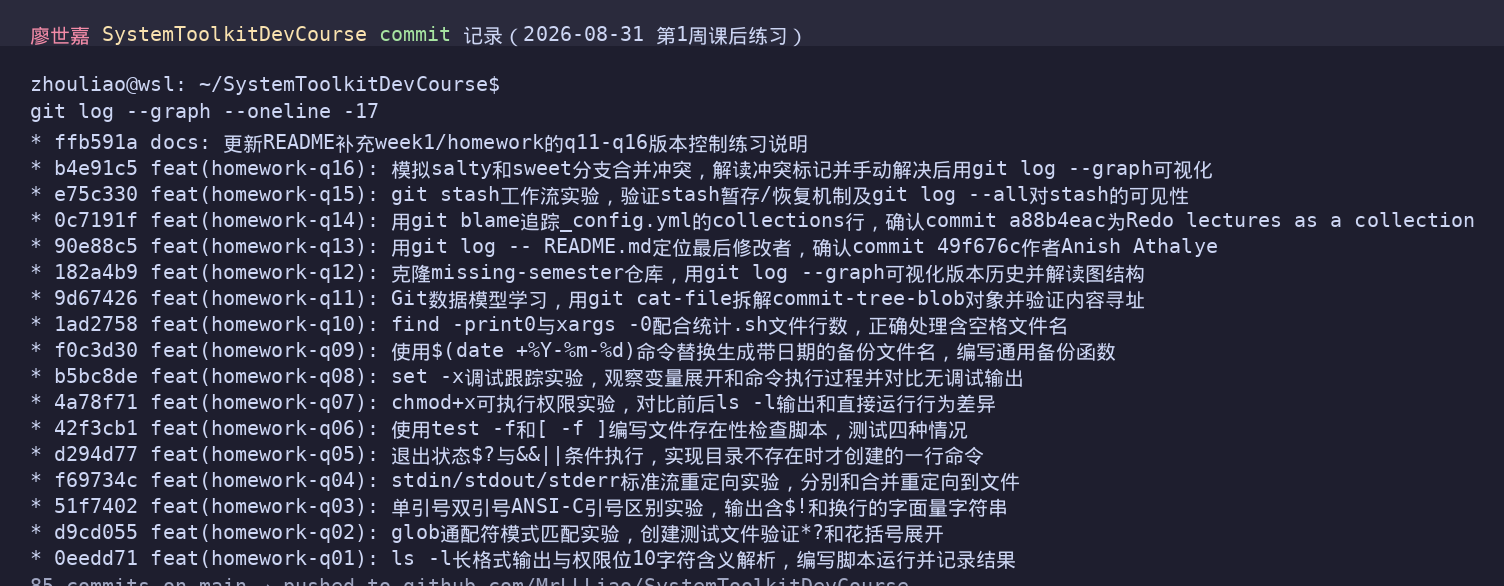
\includegraphics[width=0.92\textwidth]{commit_history.png}
\end{center}

仓库地址：\href{https://github.com/MrLLLiao/SystemToolkitDevCourse}{https://github.com/MrLLLiao/SystemToolkitDevCourse}

本周课后练习提交记录（commit 摘要）：
\begin{table}[H]
\centering
\caption{本周课后练习提交记录}
\label{tab:commits}
\begin{tabular}{clp{8.2cm}}
\toprule
哈希 & 类型 & 提交说明 \\
\midrule
0eedd71 & feat & homework-q01: ls -l 长格式与权限位解析 \\
d9cd055 & feat & homework-q02: glob 通配符模式匹配实验 \\
51f7402 & feat & homework-q03: 三种引号区别实验 \\
f69734c & feat & homework-q04: 标准流重定向实验 \\
d294d77 & feat & homework-q05: 退出状态与条件执行 \\
42f3cb1 & feat & homework-q06: test -f 文件检查脚本 \\
4a78f71 & feat & homework-q07: chmod +x 可执行权限 \\
b5bc8de & feat & homework-q08: set -x 调试跟踪 \\
f0c3d30 & feat & homework-q09: 带日期备份文件名 \\
1ad2758 & feat & homework-q10: find -print0 + xargs -0 统计行数 \\
9d67426 & feat & homework-q11: Git 数据模型与核心对象 \\
182a4b9 & feat & homework-q12: 克隆仓库并可视化版本历史 \\
90e88c5 & feat & homework-q13: 定位 README.md 最后修改者 \\
0c7191f & feat & homework-q14: git blame 追踪 collections 行 \\
e75c330 & feat & homework-q15: git stash 工作流实验 \\
b4e91c5 & feat & homework-q16: 模拟并解决 merge conflict \\
ffb591a & docs & README 补充 week1 homework q11-q16 说明 \\
\bottomrule
\end{tabular}
\end{table}

% ================= 第四部分：汇总与感悟 =================

\section{实验结果汇总}

\begin{table}[H]
\centering
\caption{本周实验与练习完成情况}
\label{tab:summary}
\begin{tabular}{clp{6.2cm}}
\toprule
编号 & 内容 & 验证结果 \\
\midrule
课上实验 & 空格文件名整理 / 日志统计 / 合并冲突 / LaTeX 文档 & 全部通过，交叉引用无 "??" \\
练习 1 & ls -l 长格式与权限位 & 10 字符含义解析正确 \\
练习 2 & glob 模式匹配 & \texttt{*} \texttt{?} \texttt{[]} 均正确匹配 \\
练习 3 & 三种引号 & 字面量 \$、!、换行安全输出 \\
练习 4 & 标准流重定向 & stdout/stderr 分流正确 \\
练习 5 & 退出状态与条件执行 & \texttt{[\ -d\ ] $||$ mkdir} 幂等验证 \\
练习 6 & test -f 脚本 & 存在/不存在分支正确 \\
练习 7 & chmod +x & 权限前后行为对比符合预期 \\
练习 8 & set -x 调试 & xtrace 输出显示变量展开 \\
练习 9 & 带日期备份 & \texttt{\$(date)} 生成正确文件名 \\
练习 10 & xargs+find 统计行数 & 含空格文件名正确处理 \\
练习 11 & Git 数据模型 & cat-file 拆解 commit/tree/blob 成功 \\
练习 12 & 可视化历史 & graph 图形解读正确 \\
练习 13 & 定位最后修改者 & commit 49f676c 定位准确 \\
练习 14 & git blame 追踪 & collections 行来源确认 \\
练习 15 & git stash 工作流 & 暂存/恢复与 --all 可见性验证 \\
练习 16 & 模拟 merge conflict & 冲突标记解读并成功解决 \\
\bottomrule
\end{tabular}
\end{table}

\section{问题与解决方法}

\subsection{Windows 与 Linux 权限命令差异}

实验初期曾在 Windows PowerShell 中执行 chmod，系统提示命令不存在。由于题目要求使用 750 和 640
这类 Unix 权限模式，因此将相关操作放到 Linux 环境下，通过 find 和 chmod 完成。

\subsection{LaTeX 中文编译问题}

使用 pdfLaTeX 直接编译包含中文姓名的文档时出现 Unicode 字符错误。之后改用 CTeX/XeLaTeX，
使中文文本和标题能够正常排版。这一问题体现了不同 TeX 引擎在字体和 Unicode 支持方面的差异。

\subsection{交叉引用检查方法}

检查 PDF 文本中的"??"时，应采用固定字符串搜索而不是容易产生歧义的正则表达式，
因此最终使用 grep -Fn '??' 进行验证。

\subsection{含空格文件名的处理（课上实验一/课后练习十）}

复制含空格文件名时，如果直接按默认换行分割会把名字拆成多个参数。课上实验一用 find -print0 |
read -d ''，课后练习十用 find -print0 | xargs -0，原理相同：以不会出现在文件名中的 null 字符
作为分隔符，从而正确处理任意文件名。这一认识贯穿后续所有文件批量处理任务。

\section{解题感悟与实验总结}

通过本次实验，我系统练习了 Linux 命令行环境中的文件管理、权限控制、Shell 管道、文本分析、
Git 分支管理和 LaTeX 文档构建。课上四个实验分别让我熟悉了隐藏文件、空格文件名和权限模式；
理解多个 Unix 文本工具通过标准输入输出构成流水线的方式；实际经历 Git 合并冲突从产生到解决的全过程；
以及强化技术文档的结构化编辑、交叉引用和自动化构建能力。

本次实验最重要的认识是：命令行任务不仅要"做出来"，还应当通过命令验证最终状态。例如，
文件权限需要通过 ls -l 或 find 检查，Shell 脚本需要检查退出码，Git 需要通过 git status 和日志
确认状态，LaTeX 则需要检查生成的 PDF 与交叉引用。通过这些验证步骤，可以显著降低操作错误并提高
实验结果的可重复性。

课后 16 个练习让我把课上实验拆解到更细的命令级能力上：引号与通配符决定了命令能否正确"表达意图"，
重定向与退出码决定了脚本能否"传递状态"，set -x 与 test 系列决定了能否"观察与判断"；
进入 Git 部分后，数据模型练习让我理解了版本控制不是"存历史"而是"内容寻址的对象图"，
stash 与冲突解决则把教科书概念变成了亲手操作过的真实工作流。这些基础练习与课上实验相互印证，
构成了完整的"操作——验证——排错"闭环。

\end{document}
